\documentclass{article}
\usepackage[utf8]{inputenc}
\usepackage[T1]{fontenc}
\usepackage{graphicx}

\title{La cueva de hielo}
\date{}
\begin{document}
\maketitle

Cathy se encuentra participando de la Inútil Olimpiada Internacional (IOI)
organizada por la Organización Cultural de Internet (OCI). En una de las
competencias, los participantes deben completar el laberinto de la cueva de
hielo de cierta franquicia de criaturas de bolsillo. Rápidamente, Cathy nota que
la organización ha modificado los laberintos y las soluciones que había
memorizado no le servirán. Sin embargo, las mecánicas del laberinto se
conservan. Es decir,
\begin{itemize}
	\item cada casilla que el personaje debe moverse toma una unidad de tiempo
	\item como el piso es de hielo, al moverse en una dirección, el personaje
	debe continuar hasta chocar con una roca o una muralla
	\item tanto la entrada como la salida del laberinto están en los bordes de éste.
\end{itemize}

En la figura se muestra un camino que toma $7 + 2 + 4 + 3 + 1 + 2 + 9 = 28$
unidades de tiempo para llegar a la salida.
\begin{center}
	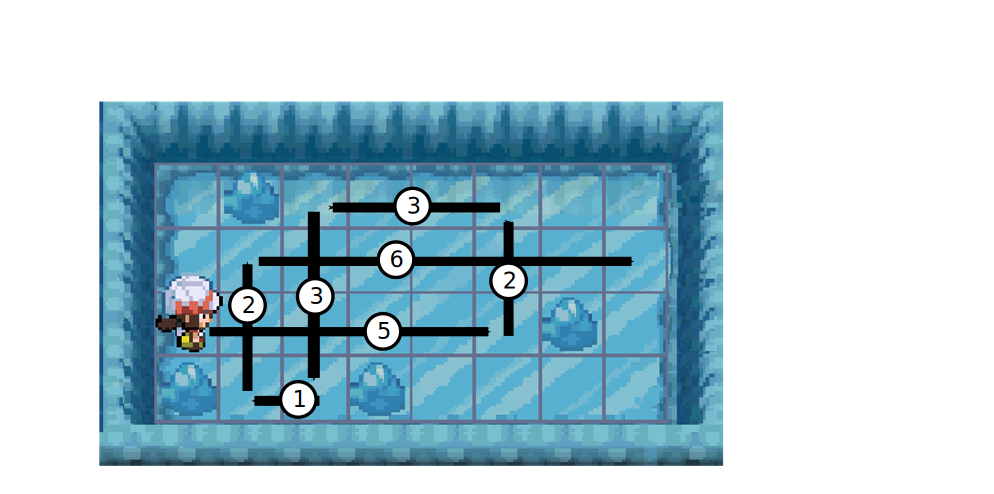
\includegraphics[width=0.95\textwidth]{ice2.png}
\end{center}

¿Puedes ayudar a Cathy a encontrar los mejores tiempos posibles para cada
laberinto?

\section*{Entrada}
Cada caso de prueba parte con una línea con dos enteros $R$ y $C$. A
continuación, hay $R$ líneas cada una con $C$ símbolos. \texttt{E} corresponde
a la entrada, \texttt{S} a la salida, \texttt{*} a un roca o muralla y
\texttt{.} al piso de hielo.

\section*{Salida}
Un entero con el menor tiempo posible para resolver el laberinto o \texttt{-1}
si no es posible resolverlo.
\end{document}
